
\begin{aufgabe}
	Bestimmen Sie den Schwerpunkt der folgenden Körper.

	\begin{center}
	
\begin{tikzpicture}
	\def\DX{4}%in x richtung
	\def\DY{4}%in y richtung
	\def\DB{1}%breite
	\draw (0,0) node [above left] {a)};
	\fill [color=black!30] (0,0)--++(\DX,0)--++(0,-\DB)--++(-\DX+\DB,0)--++(0,-\DY+\DB)--++(-\DB,0)--(0,0);
	
	\def\DX{5}%in x richtung
	\def\DY{6}%in y richtung
	\def\DB{1.5}%breite
	\draw (8,0) node [above left] {b)};
	\fill [color=black!30] (8,0)--++(\DX,0)--++(0,-\DB)--++(-\DX+\DB,0)--++(0,-\DY+\DB)--++(-\DB,0)--(8,0);


	\end{tikzpicture}
	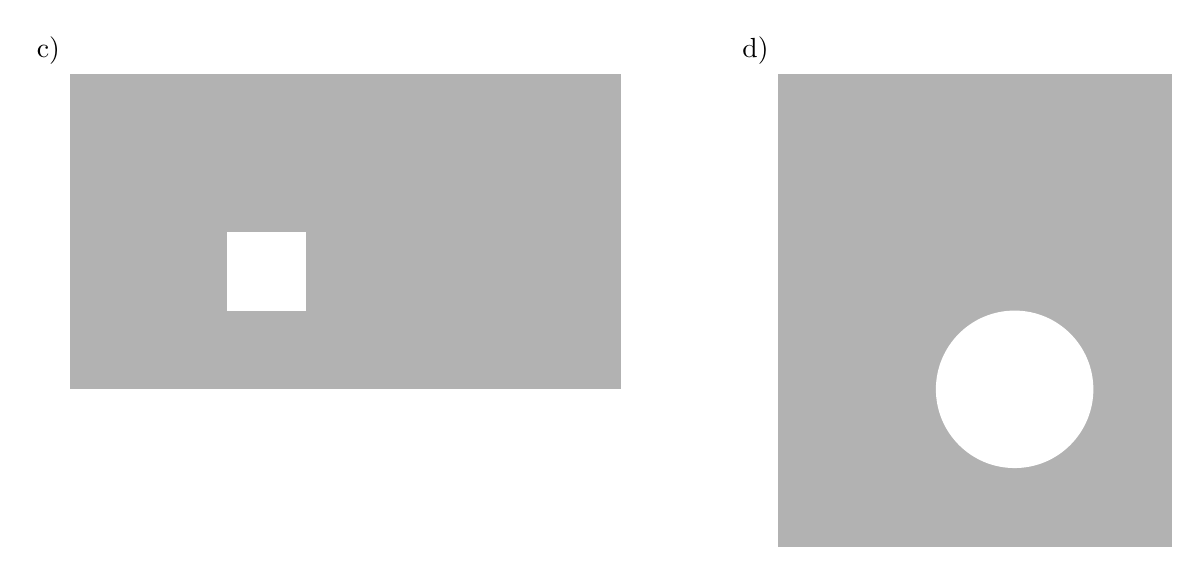
\begin{tikzpicture}
	\draw (0,0) node [above left] {c)};
	\fill [color=black!30] (0,0) rectangle (7,-4);
	\fill [color=white] (2,-2) rectangle (3,-3);


	\draw (9,0) node [above left] {d)};
	\fill [color=black!30] (9,0) rectangle (14,-6);
	\fill [color=white] (12,-4) circle (1cm);

\end{tikzpicture}
	\end{center}
\end{aufgabe}

